\section{Multiple injection points}
The \confignoc{} has a single injection point and only allows for the transmission of a single message at a time.
Thus, when transmitting data from external memory to a neuron core, only a fraction of the NoC's capacity is in use and the remaining part  is left unused.
Also, cores are configured sequentially.
There is a significant potential to improve the utilization of the NoC and parallelism to reduce the configuration time.
We propose to divide the NoC into multiple independent zones.
Each zone is a collection of adjacent clusters including the links between them (example segmentations are illustrated in \cref{fig:segmentation_example}).
Each of the zones is accompanied by a separate interface to the external world, allowing each zone to have data injected into its cores separately and in parallel to other zones.
Having more zones will allow for more parallel data transfers.
To maximize the throughput, the zones should not overlap with each other.
Otherwise, traffic originating from two different sources may cause congestion in the network. 
As a result of this change, the total bandwidth will increase, lowering the end-to-end latency.

We study the effects on performance when introducing multiple injection points.
For three different phit widths and a variety of zones, we compute the latency for sending \SI{36}{MiB} to the \graicore{}.
The results are shown in \cref{fig:zones_vs_latency_vs_phit_width} for the old and new packet format.

\begin{figure}[htbp]
    \centering
    \begin{subfigure}[b]{0.48\textwidth}
        \begin{adjustbox}{width=\linewidth}
            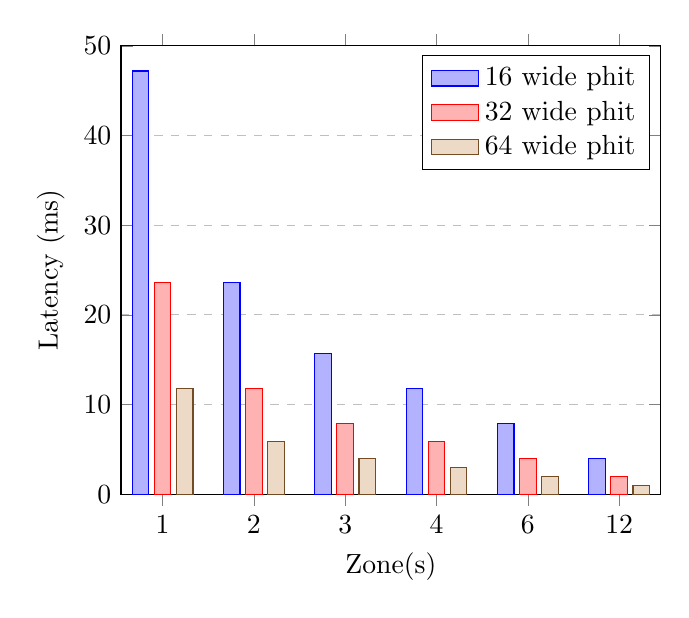
\begin{tikzpicture}
\begin{axis}[
    ylabel=Latency (ms),
    xlabel=Zone(s),
    ymajorgrids=true,
    grid style=dashed,
    ymin=0, ymax=50,
    symbolic x coords={1, 2, 3, 4, 6, 12},
    xtick={1, 2, 3, 4, 6, 12},
    ybar,
    enlarge x limits={abs=15pt},
    bar width=6pt
]

\addplot+[
area legend,
] 
    coordinates {
        (1,47.19)
        (2,23.59)
        (3,15.73)
        (4,11.80)
        (6,7.86)
        (12,3.93)
    };
\addplot+[
area legend,
] 
    coordinates {
        (1,23.59)
        (2,11.80)
        (3,7.86)
        (4,5.90)
        (6,3.93)
        (12,1.97)
    };
\addplot+[
area legend,
] 
    coordinates {
        (1,11.80)
        (2,5.90)
        (3,3.93)
        (4,2.95)
        (6,1.97)
        (12,0.98)
    };
\legend{16 wide phit, 32 wide phit, 64 wide phit}
\end{axis}
\end{tikzpicture}
        \end{adjustbox}
        \caption{Old packet format}
        % \label{}
    \end{subfigure}
    \hfill
    \begin{subfigure}[b]{0.48\textwidth}
        \begin{adjustbox}{width=\linewidth}
            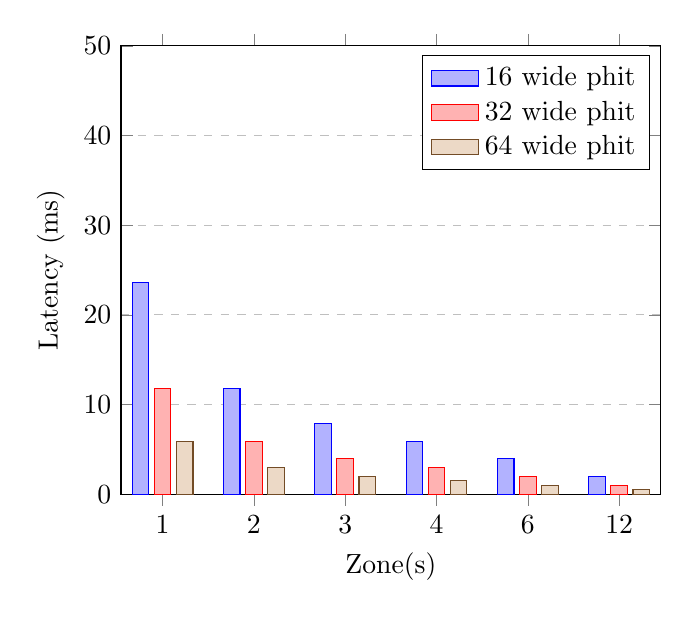
\begin{tikzpicture}
\begin{axis}[
    ylabel=Latency (ms),
    xlabel=Zone(s),
    ymajorgrids=true,
    grid style=dashed,
    ymin=0, ymax=50,
    symbolic x coords={1, 2, 3, 4, 6, 12},
    xtick={1, 2, 3, 4, 6, 12},
    ybar,
    enlarge x limits={abs=15pt},
    bar width=6pt
]

\addplot+[
area legend,
] 
	coordinates {
            (1,23.59)
            (2,11.80)
            (3,7.86)
            (4,5.90)
            (6,3.93)
            (12,1.97)
        };
\addplot+[
area legend,
] 
	coordinates {
            (1,11.80)
            (2,5.90)
            (3,3.93)
            (4,2.95)
            (6,1.97)
            (12,0.98)
        };
\addplot+[
area legend,
] 
	coordinates {
            (1,5.90)
            (2,2.95)
            (3,1.97)
            (4,1.47)
            (6,0.98)
            (12,0.49)
        };
\legend{16 wide phit, 32 wide phit, 64 wide phit}
\end{axis}
\end{tikzpicture}
        \end{adjustbox}
        \caption{New packet format}
        % \label{}
    \end{subfigure}
    \caption[]{The effects of the number of zones and phit width on the latency}
    \label{fig:zones_vs_latency_vs_phit_width}
\end{figure}


Similar to the increase of the phit width, we observe that the number of zones and latency are inversely proportional. While the number of zones and bandwidth are directly proportional.

\begin{figure}[htbp]
    \centering
    \begin{subfigure}[b]{0.48\linewidth}
        \centering
        \begin{adjustbox}{width=0.6\linewidth}
            \begin{tikzpicture}[]
    \draw (-0.5, 0) -- (0, 0);
    \node [diamond, draw, fill=purple] () at (-0.5,0) {};
    
    \draw (0, 0) grid[step=0.5] (5.5,5.5);
    \foreach \x in {0,...,11} {
        \foreach \y in {0,...,11} {
           \node [circle, draw, fill=red] (\x\y) at (0.5*\x,0.5*\y) {};
        }
    }
\end{tikzpicture}
        \end{adjustbox}
        \caption{One zone}
        \label{fig:segmentation_example_1}
    \end{subfigure}
    \hfill
    \begin{subfigure}[b]{0.48\linewidth}
        \centering
        \begin{adjustbox}{width=0.6\linewidth}
            \begin{tikzpicture}[]
    \draw (-0.5, 3) -- (0, 3);
    \node [diamond, draw, fill=purple] () at (-0.5,3) {};
    
    \draw (-0.5, 0) -- (0, 0);
    \node [diamond, draw, fill=purple] () at (-0.5,0) {};
    
    \draw (0, 0) grid[step=0.5] (5.5,5.5);
    \foreach \x in {0,...,11} {
        \foreach \y in {0,...,5}  {
           \node [circle, draw, fill=red] (\x\y) at (0.5*\x,0.5*\y) {};
        }
        \foreach \y in {6,...,11} {
           \node [circle, draw, fill=blue] (\x\y) at (0.5*\x,0.5*\y) {};
        }
    }
\end{tikzpicture}

        \end{adjustbox}
        \caption{Two zones}
        \label{fig:segmentation_example_2}
    \end{subfigure}
    \\ \vspace{1.5em}
    \begin{subfigure}[b]{0.48\linewidth}
        \centering
        \begin{adjustbox}{width=0.6\linewidth}
            \begin{tikzpicture}[]
    \draw (-0.5, 4) -- (0, 4);
    \node [diamond, draw, fill=purple] () at (-0.5,4) {};
    
    \draw (-0.5, 2) -- (0, 2);
    \node [diamond, draw, fill=purple] () at (-0.5,2) {};
    
    \draw (-0.5, 0) -- (0, 0);
    \node [diamond, draw, fill=purple] () at (-0.5,0) {};
    
    \draw (0, 0) grid[step=0.5] (5.5,5.5);
    \foreach \x in {0,...,11} {
        \foreach \y in {0,...,3}  {
           \node [circle, draw, fill=red] (\x\y) at (0.5*\x,0.5*\y) {};
        }
        \foreach \y in {4,...,7} {
           \node [circle, draw, fill=blue] (\x\y) at (0.5*\x,0.5*\y) {};
        }
        \foreach \y in {8,...,11} {
           \node [circle, draw, fill=green] (\x\y) at (0.5*\x,0.5*\y) {};
        }
    }
\end{tikzpicture}

        \end{adjustbox}
        \caption{Three zones}
        \label{fig:segmentation_example_3}
    \end{subfigure}
    \hfill
    \begin{subfigure}[b]{0.48\linewidth}
        \centering
        \begin{adjustbox}{width=0.6\linewidth}
            \begin{tikzpicture}[]
    \draw (-0.5, 4.5) -- (0, 4.5);
    \node [diamond, draw, fill=purple] () at (-0.5,4.5) {};
    
    \draw (-0.5, 3) -- (0, 3);
    \node [diamond, draw, fill=purple] () at (-0.5,3) {};
    
    \draw (-0.5, 1.5) -- (0, 1.5);
    \node [diamond, draw, fill=purple] () at (-0.5,1.5) {};
    
    \draw (-0.5, 0) -- (0, 0);
    \node [diamond, draw, fill=purple] () at (-0.5,0) {};
    
    \draw (0, 0) grid[step=0.5] (5.5,5.5);
    \foreach \x in {0,...,11} {
        \foreach \y in {0,...,2}  {
           \node [circle, draw, fill=red] (\x\y) at (0.5*\x,0.5*\y) {};
        }
        \foreach \y in {3,...,5} {
           \node [circle, draw, fill=blue] (\x\y) at (0.5*\x,0.5*\y) {};
        }
        \foreach \y in {6,...,8} {
           \node [circle, draw, fill=green] (\x\y) at (0.5*\x,0.5*\y) {};
        }
        \foreach \y in {9,...,11} {
           \node [circle, draw, fill=yellow] (\x\y) at (0.5*\x,0.5*\y) {};
        }
    }
\end{tikzpicture}
        \end{adjustbox}
        \caption{Four zones}
        \label{fig:segmentation_example_4}
    \end{subfigure}
    \caption{
    Example segmentation of the \confignoc{} into multiple zones.
    A zone is a set of nodes (circle) and is illustrated by a distinct color.
    The arrows show the unique injection sources for each zone.
    }
    \label{fig:segmentation_example}
\end{figure}

